\chapter{Tabular benchmarks specification and results}
\label{ch:tabular}

\begin{table}[H]
    \centering
\begin{tabular}{ccccc}
    \hline
    \textbf{Benchmark} & \textbf{Epochs} & \textbf{1x full eval (s)} & \textbf{Max t (s)} & \textbf{Full evals} \\ \hline
    lc-Fashion-MNIST & 50 & 1200 & 7200 & 6 \\ \hline
    lc-airlines & 50  & 1108 & 7200  & 6.5 \\ \hline
    lc-albert  & 50  & 934  & 7200 & 7.7 \\ \hline
    lc-covertype  & 50  & 650  & 7200  & 11  \\ \hline
    lc-christine  & 50  & 2376  & 7200  & 3  \\ \hline
    nas-cifar100 & 200 & 3649  & 21600  & 5.9 \\ \hline
    nas-cifar10  & 200 & 3649  & 18000 & 4.9 \\ \hline
    nas-ImageNet & 200 & 10450 & 28800 & 2.7 \\ \hline
    fc-protein & 100 & 254  & 3600  & 14.1 \\ \hline
    fc-naval  & 100  & 68  & 3600  & 53 \\ \hline
    fc-parkinsons  & 100  & 33.9 & 3600  & 109 \\ \hline
    fc-slice  & 100  & 354 & 3600  & 10 \\ \hline
\end{tabular}
\caption{Summary of the tabular benchmarks.}
\end{table}


\begin{table}
    \centering
\begin{tabular}{cc}
    \textbf{Hyperparameter} & \textbf{Values} \\ \midrule
    Batch size & $\{16, 512\}$ \\
    Learning rate & $\{1\mathrm{e}{-4}, 1\mathrm{e}{-1}\}$ \\
    Momentum & $\{0.1, 0.99\}$ \\
    Weight decay & $\{1\mathrm{e}{-5}, 1\mathrm{e}{-1}\}$ \\
    Layers & $\{1, 5\}$ \\
    Max units/layer & $\{64, 1024\}$ \\
    Dropout & $\{0.0, 1.0\}$
    \end{tabular}
    \caption{LCBench hyperparameter values}
    \label{tab:lc}
\end{table}

\begin{table}
    \centering
\begin{tabular}{cc}
    \textbf{Hyperparameter} & \textbf{Values} \\ \midrule
    Learning rate & $\{0.0005, 0.001, 0.005, 0.01, 0.05, 0.1\}$ \\
    Batch size & $\{8, 16, 32, 64\}$ \\
    LR schedule & $\{$cosine, fix $\}$ \\
    Activation L1 & $\{$relu, tanh $\}$ \\
    Activation L2 & $\{$relu, tanh $\}$ \\
    L1 size & $\{8, 16, 32, 64, 128, 256, 512\}$ \\
    L2 size & $\{8, 16, 32, 64, 128, 256, 512\}$ \\
    Dropout L1 & $\{0.0, 0.3, 0.6\}$ \\
    Dropout L2 & $\{0.0, 0.3, 0.6\}$
    \end{tabular}
    \caption{FCNet hyperparameter values}
    \label{tab:fcnet}
\end{table}


%Tabular benchmarks for joint architecture and hyperparameter optimization. Klein, A. and Hutter, F. 2019.
\begin{figure}[H]
    \centering
    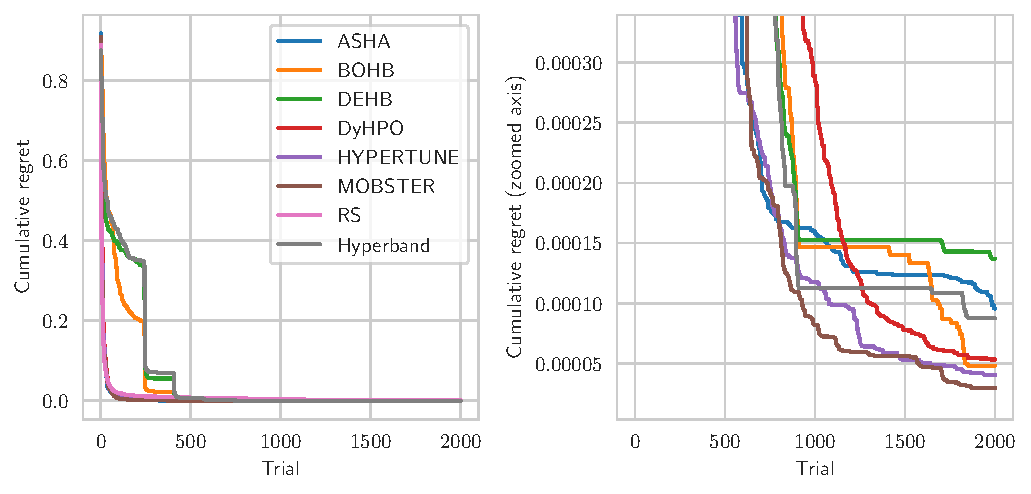
\includegraphics[scale=0.58]{img/tabular_exp/fcnet-naval_plot.pdf}
    \caption{FCNet-naval}
    %\label{}
\end{figure}

\begin{figure}[H]
    \centering
    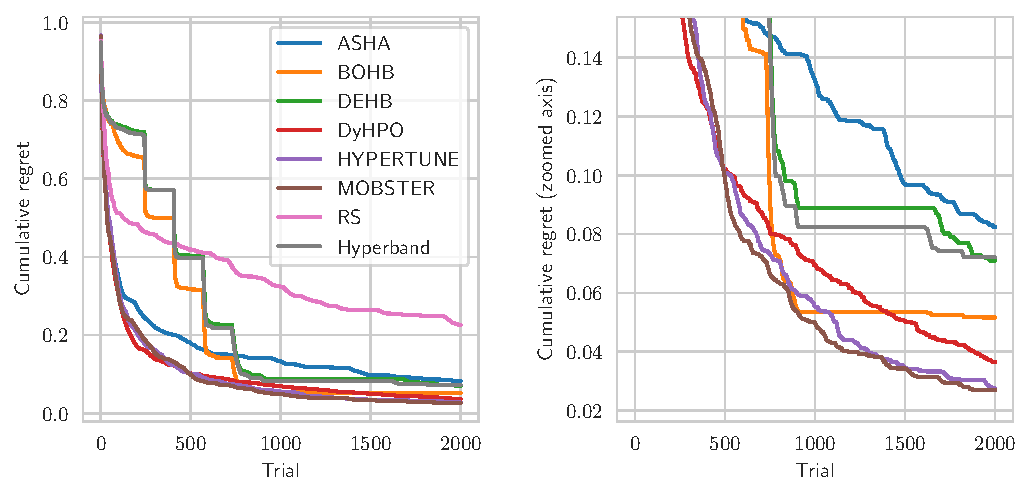
\includegraphics[scale=0.58]{img/tabular_exp/fcnet-protein_plot.pdf}
    \caption{FCNet-protein}
    %\label{}
\end{figure}


\begin{figure}[H]
    \centering
    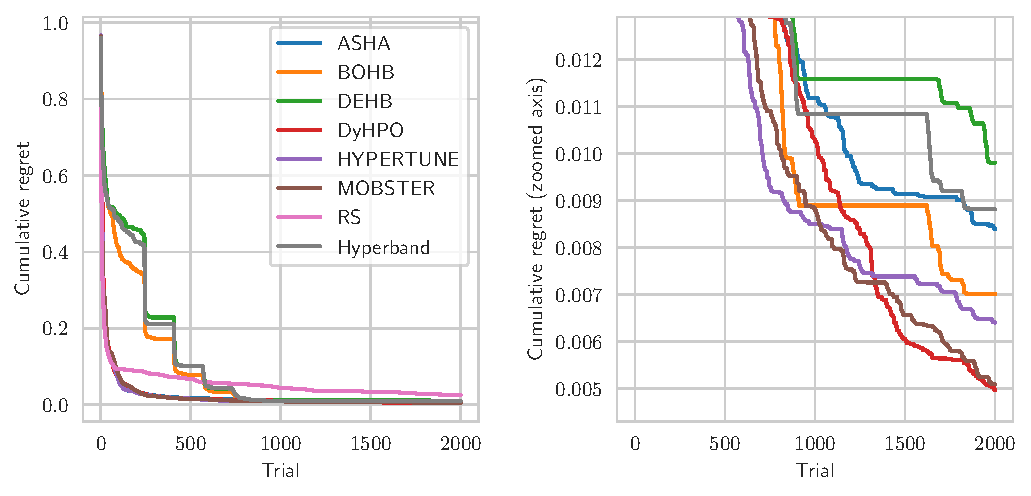
\includegraphics[scale=0.58]{img/tabular_exp/fcnet-parkinsons_plot.pdf}
    \caption{FCNet-parkinsons}
    %\label{}
\end{figure}

\begin{figure}[H]
    \centering
    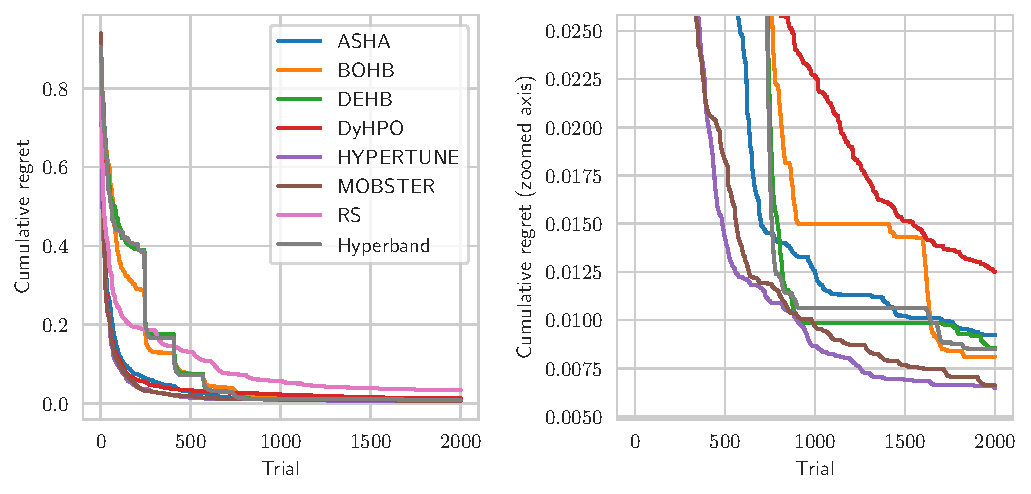
\includegraphics[scale=0.58]{img/tabular_exp/fcnet-slice_plot.pdf}
    \caption{FCNet-slice}
    %\label{}
\end{figure}




% NAS-Bench-201: Extending the scope of reproducible neural architecture search. Dong, X. and Yang, Y. 2020.
\begin{figure}[H]
    \centering
    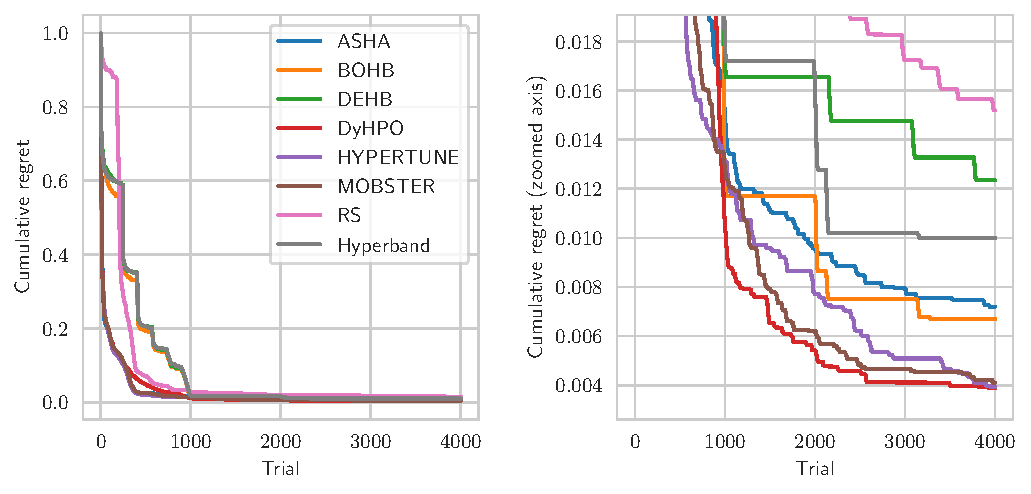
\includegraphics[scale=0.58]{img/tabular_exp/nas201-cifar10_plot.pdf}
    \caption{nas201-cifar10}
    %\label{}
\end{figure}

\begin{figure}[H]
    \centering
    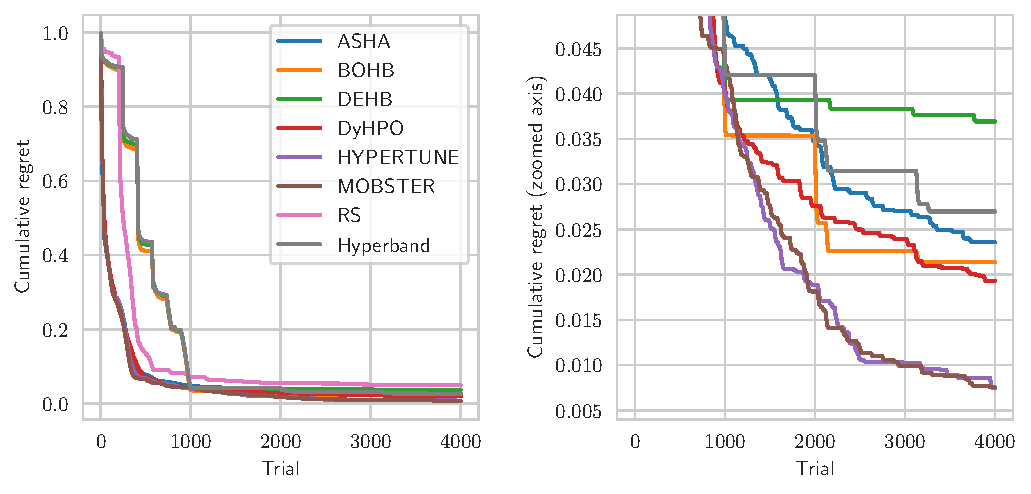
\includegraphics[scale=0.58]{img/tabular_exp/nas201-cifar100_plot.pdf}
    \caption{nas201-cifar100}
    %\label{}
\end{figure}

\begin{figure}[H]
    \centering
    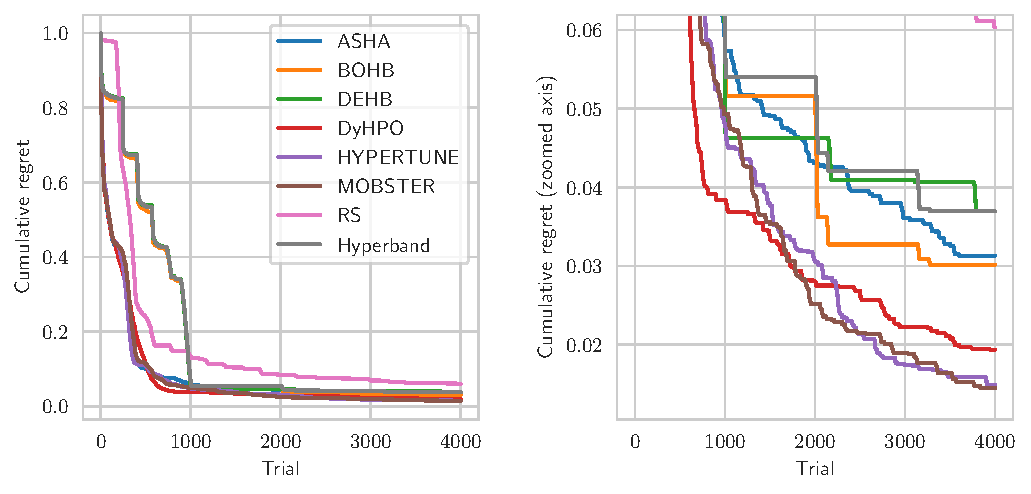
\includegraphics[scale=0.58]{img/tabular_exp/nas201-ImageNet16-120_plot.pdf}
    \caption{nas201-ImageNet16-120}
    %\label{}
\end{figure}

%Reference: Auto-PyTorch: Multi-Fidelity MetaLearning for Efficient and Robust AutoDL. Lucas Zimmer, Marius Lindauer, Frank Hutter. 2020.
\begin{figure}[H]
    \centering
    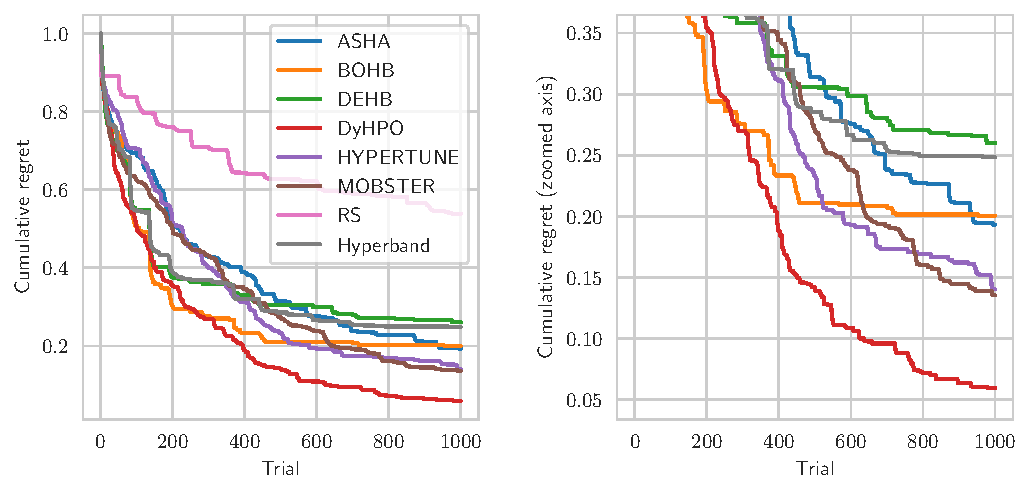
\includegraphics[scale=0.58]{img/tabular_exp/lcbench-airlines_plot.pdf}
    \caption{LCBench-airlines}
    %\label{}
\end{figure}

\begin{figure}[H]
    \centering
    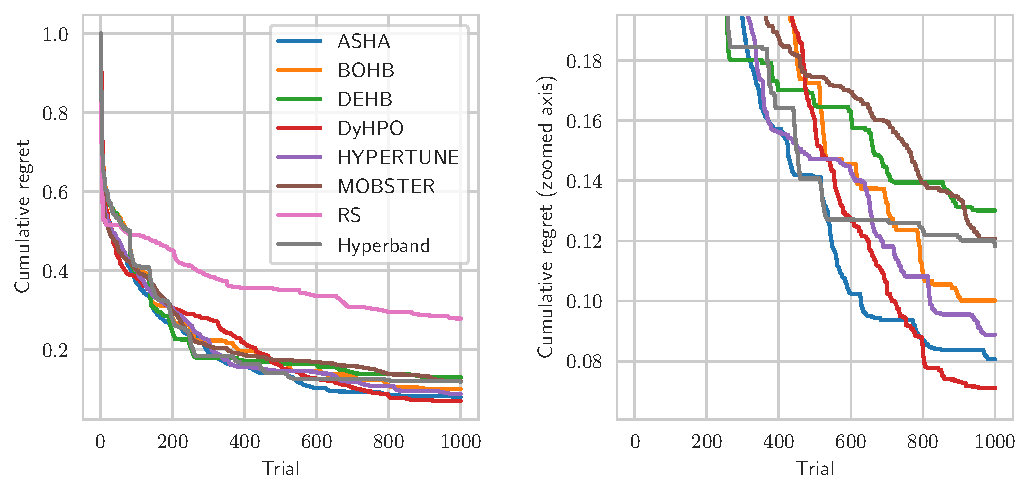
\includegraphics[scale=0.58]{img/tabular_exp/lcbench-albert_plot.pdf}
    \caption{LCBench-albert}
    %\label{}
\end{figure}

\begin{figure}[H]
    \centering
    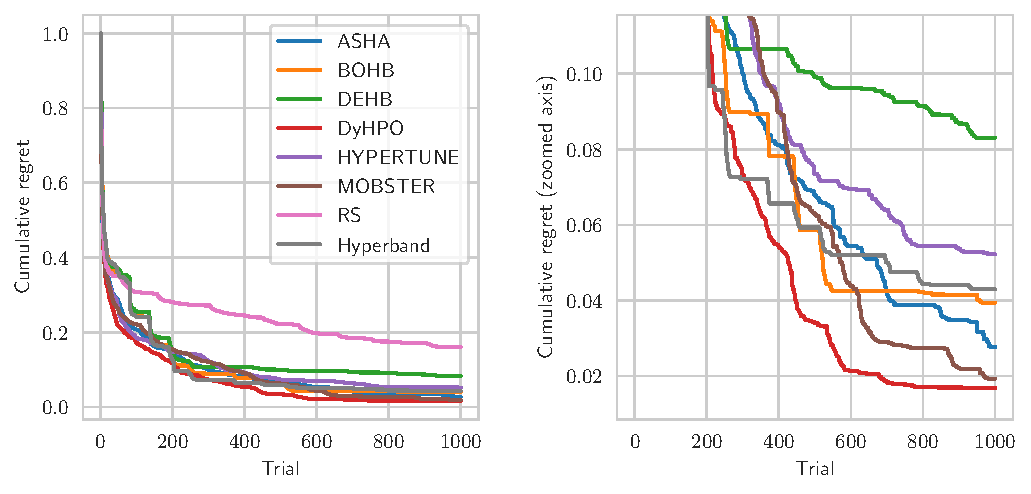
\includegraphics[scale=0.58]{img/tabular_exp/lcbench-Fashion-MNIST_plot.pdf}
    \caption{LCBench-Fashion-MNIST}
    %\label{}
\end{figure}

\begin{figure}[H]
    \centering
    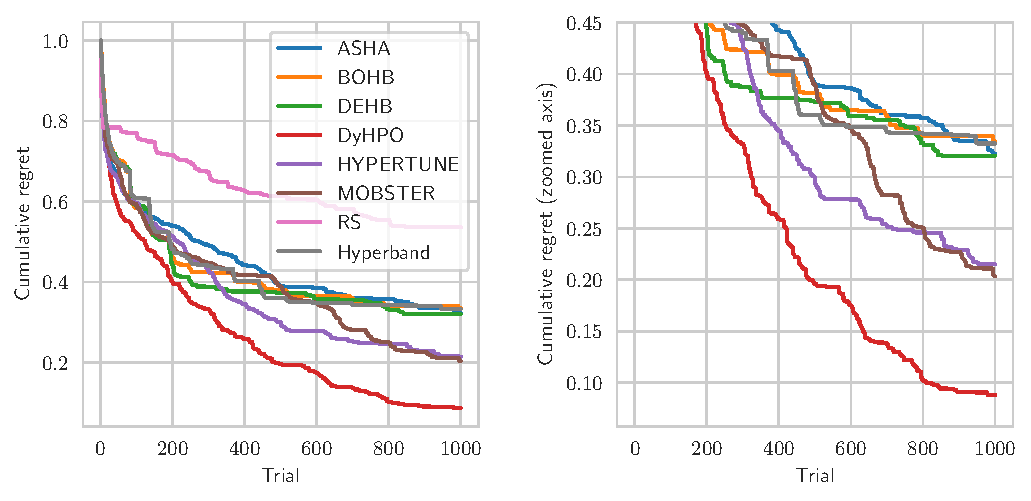
\includegraphics[scale=0.58]{img/tabular_exp/lcbench-covertype_plot.pdf}
    \caption{LCBench - covertype}
    %\label{}
\end{figure}

\begin{figure}[H]
    \centering
    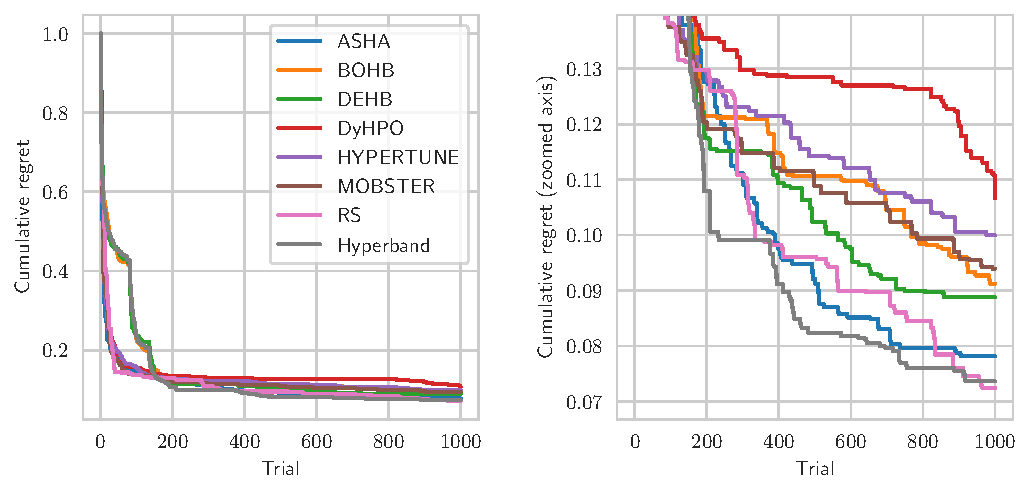
\includegraphics[scale=0.58]{img/tabular_exp/lcbench-christine_plot.pdf}
    \caption{LCBench-christine}
    %\label{}
\end{figure}
